\documentclass[aspectratio=169,11pt,usenames,dvipsnames,handout]{beamer}

\usepackage[czech,english]{babel}
\usepackage{CJKutf8}
\newcommand{\zh}[1]{\begin{CJK}{UTF8}{gbsn}#1\end{CJK}}
\usepackage{graphicx}
\usepackage{enumitem}
\usepackage{amsmath}
\newlength{\dhatheight}
\newcommand{\doublehat}[1]{%
    \settoheight{\dhatheight}{\ensuremath{\hat{#1}}}%
    \addtolength{\dhatheight}{-0.2ex}%
    \hat{\vphantom{\rule{1pt}{\dhatheight}}%
    \smash{\hat{#1}}}}
\usepackage{mathtools}
\usepackage{float}
\usepackage{tikz}
\usetikzlibrary{patterns,arrows.meta,calc,3d,angles}
\usepackage{tkz-euclide}
\tikzset{point style/.style = {%
  draw = black,
  inner sep = 0pt,
  shape = circle,
  minimum size = 5pt,
  fill = black
 }
}
\usepackage{enumitem}

\usepackage{caption}
\usepackage{subcaption}

\usepackage{booktabs}
% Flowchart stuff

\usepackage{pgfopts}
\usepackage{xcolor}
\usepackage{tcolorbox}

\usetheme[
 titlestyle=style2,
 titleformat=smallcaps,
 sectionstyle=plain,
 slidestyle=cyber,
 headingcolor=theme,
 block=transparent
]{trigon}

\title{Systems of Linear Equations}
\date{\today}
\author{Adam Klepáč}
\institute[GEVO]{Gymnázium Evolution Jižní Město}
\biglogo[width=.2\textwidth]{logo}
\smalllogo[width=.1\textwidth]{logo}
\titlegraphic{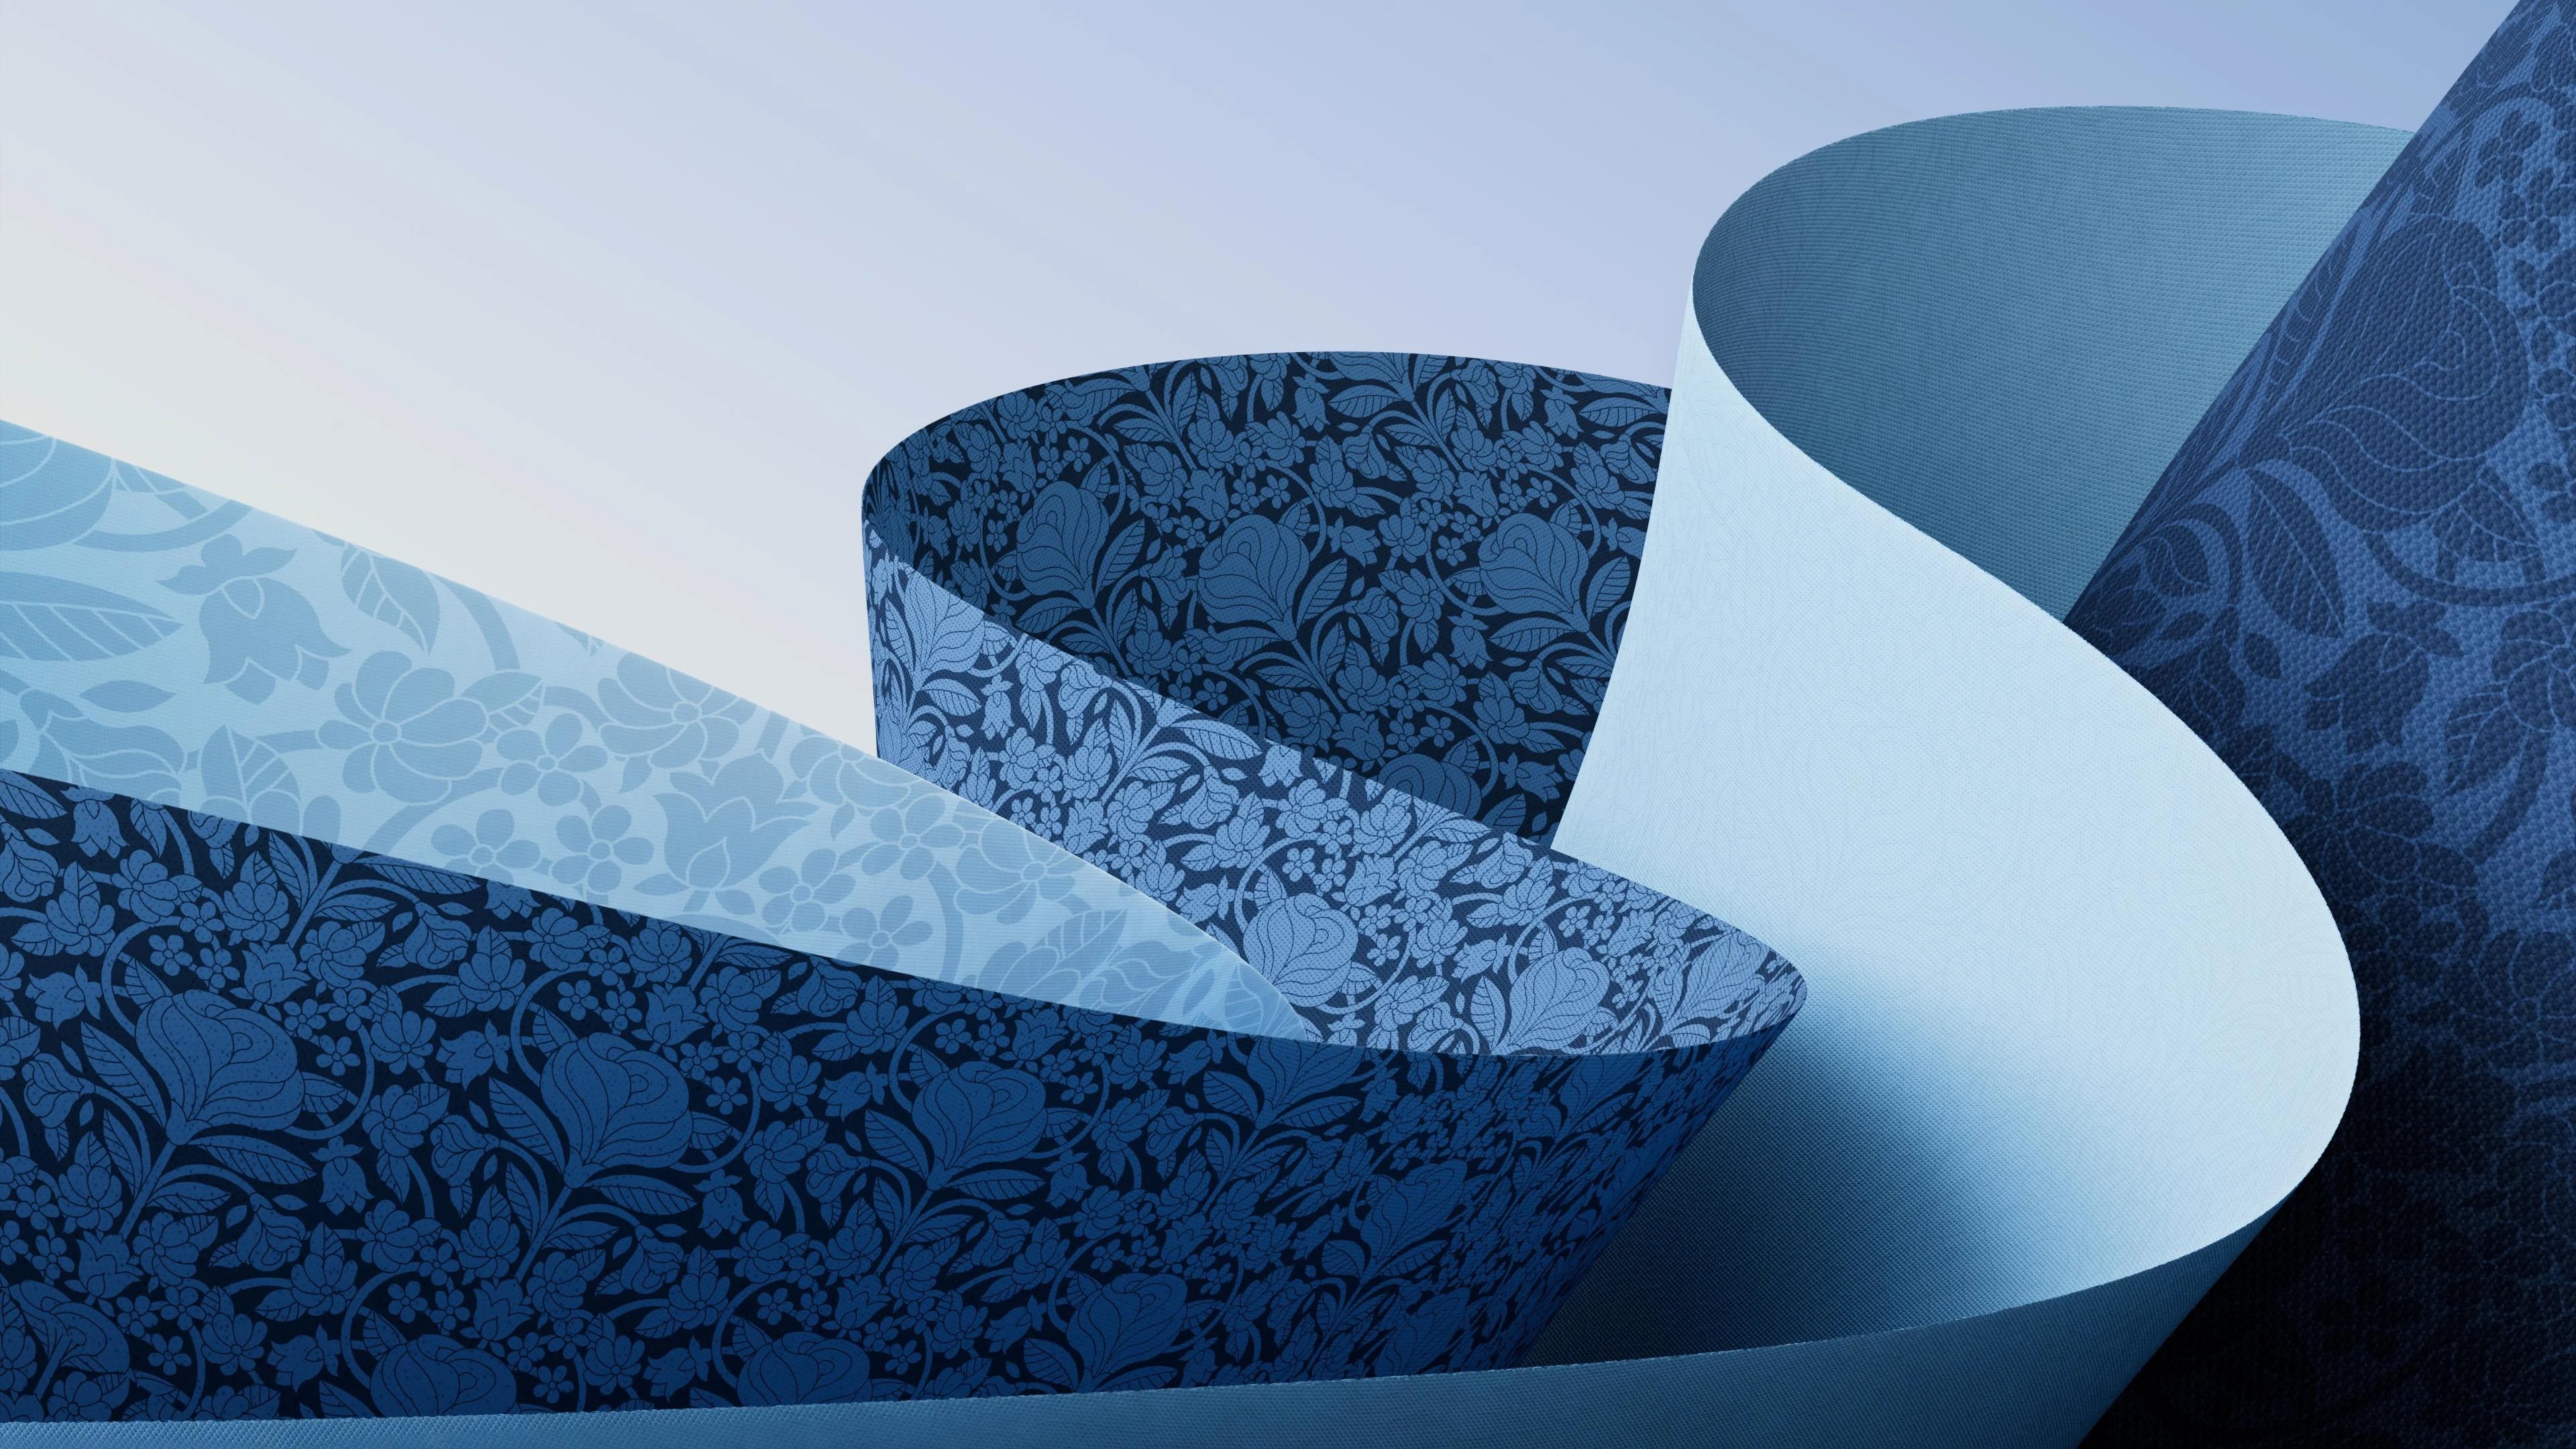
\includegraphics[height=\paperheight]{title}}

\def\subsectionname{}

% enumerate and itemize global settings
\setlist{topsep=0pt}
\setlist[itemize,1]{label=\textbullet}
\setlist[itemize,2]{label=\textopenbullet}
\setlist[enumerate,1]{label=\arabic*.}
\setlist[enumerate,2]{label=\alph*)}

% custom colors %
\definecolor{RichBlack}{HTML}{050F1F}
\definecolor{PowderBlue}{HTML}{9ABBD8}
\definecolor{BlueGray}{HTML}{6897BE}
\definecolor{BerkeleyBlue}{HTML}{092B55}
\definecolor{LapisLazuli}{HTML}{40698F}

\colorlet{tPrim}{BerkeleyBlue}
\colorlet{tTheme}{PowderBlue}
\colorlet{tSec}{LapisLazuli}
\colorlet{tAccent}{BlueGray}
\colorlet{tText}{RichBlack}

\newcommand{\clr}{\textcolor{BrickRed}}
\newcommand{\clb}{\textcolor{RoyalBlue}}
\newcommand{\clg}{\textcolor{ForestGreen}}
\newcommand{\clm}{\textcolor{Magenta}}
\newcommand{\cls}{\textcolor{Salmon}}
\newcommand{\clo}{\textcolor{OrangeRed}}

\newcommand{\N}{\mathbb{N}}
\newcommand{\Z}{\mathbb{Z}}
\renewcommand{\P}{\mathbb{P}}
\DeclareMathOperator{\tng}{\triangle}
\DeclareMathOperator{\dv}{div}

\tcbset{
 boxsep=7pt,
 fonttitle=\sc,
 colframe=tGreyBg,
 colframe=tSec,
 boxrule=1pt
}

\begin{document}
\titleframe

\begin{frame}
 \frametitle{Contents}
 \tableofcontents
\end{frame}

\section{Functions}

\begin{frame}
 \frametitle{What Is A Function?}
 Intuitively, a function is a \alert{box} which receives data and gives some
 data back.\pause
 \begin{center}
  \begin{tikzpicture}
   \node[draw,rectangle,minimum height=1cm,minimum
    width=2cm,color=BlueGray,align=center] (f)
    at (0,0) {function \\ \footnotesize `\emph{do something with \clr{input}'}};
   \node[left=2cm of f] (in) {\clr{input}};
   \node[right=2cm of f] (out) {\clb{output}};
   \draw[-latex,thick,shorten <= 2pt, shorten >= 2pt] (in) -- (f);
   \draw[-latex,thick,shorten <= 2pt, shorten >= 2pt] (f) -- (out);
  \end{tikzpicture}
 \end{center}
 \pause
 We'll call the data that \alert{a function receives}, \clr{inputs} and the
 \alert{data it gives back}, \clb{outputs}. \\ \pause
 \clr{Inputs} and \clb{outputs} need not necessarily be just `one object', they
 can be for example lists of numbers.
\end{frame}

\begin{frame}
 \frametitle{Functions -- Example}
 A function which returns the \alert{average} of a given set of numbers receives
 the numbers and also their count as \clr{input} and returns the \alert{average}
 as \clb{output}.\pause
 \begin{center}
  \begin{tikzpicture}
   \node[draw,rectangle,minimum height=1cm,minimum
    width=2cm,color=BlueGray,align=center] (f)
    at (0,0) {average \\ \footnotesize `\emph{sum all the numbers}\\
     \footnotesize \emph{and
    divide them by $n$}'};
   \node[left=2cm of f,align=center] (in)
    {\clr{$x_1,x_2,\ldots,x_n$}\\\clr{$n$}}; \node[right=2cm of f] (out)
     {\clb{$\displaystyle \frac{x_1+x_2+\ldots +x_n}{n}$}};
   \draw[-latex,thick,shorten <= 2pt, shorten >= 2pt] (in) -- (f);
   \draw[-latex,thick,shorten <= 2pt, shorten >= 2pt] (f) -- (out);
  \end{tikzpicture}
 \end{center}
\end{frame}

\begin{frame}
 \frametitle{Functions -- Example}
 We can also consider `non-mathematical' functions. Like a function which
 receives a type of meal and returns the ingredients.\\ \pause
 \begin{center}
  \begin{tikzpicture}
   \node[draw,rectangle,minimum height=1cm,minimum
    width=2cm,color=BlueGray,align=center] (f) at (0,0) {ingredients};
   \node[left=2cm of f,align=center] (in) {\clr{omelette}};
   \node[right=2cm of f,align=center] (out) {\clb{eggs} \\ \clb{salt} \\
    \clb{butter}};
   \draw[-latex,thick,shorten <= 2pt, shorten >= 2pt] (in) -- (f);
   \draw[-latex,thick,shorten <= 2pt, shorten >= 2pt] (f) -- (out);
  \end{tikzpicture}
 \end{center}
\end{frame}

\subsection{Function Composition}

\begin{frame}
 \subsectionpage
\end{frame}

\begin{frame}
 \frametitle{Function Composition}
 If we have \alert{two functions}, we can \alert{in certain cases} `compose'
 them. \\ \pause
 \alert{Composition} simply means that \alert{one function follows the other} --
 in other words, the \clb{output} of the first function is the \clr{input} of
 the second.\\ \pause
 Of course, \alert{composition} is only possible if the \clb{output} of the
 first function is a valid \clr{input} for the second. \\ \pause
 For instance, you could hardly compose the \alert{ingredients} function with
 the \alert{average} function.
\end{frame}

\begin{frame}
 \frametitle{Function Composition}
 Considering two functions
 \vspace*{-1em}
 \begin{center}
  \begin{tikzpicture}
   \node[draw,rectangle,minimum height=.5cm,minimum
    width=2cm,color=BlueGray,align=center] (f) at (0,0) {sum};
   \node[left=2cm of f,align=center] (in) {\clr{$a,b$}};
   \node[right=2cm of f,align=center] (out) {\clb{$a + b$}};
   \draw[-latex,thick,shorten <= 2pt, shorten >= 2pt] (in) -- (f);
   \draw[-latex,thick,shorten <= 2pt, shorten >= 2pt] (f) -- (out);

   \node[draw,rectangle,minimum height=.5cm,minimum
    width=2cm,color=BlueGray,align=center,below=.5cm of sum] (g) {times two};
   \node[left=2cm of g,align=center] (in) {\clr{$a$}};
   \node[right=2cm of g,align=center] (out) {\clb{$2 \cdot a$}};
   \draw[-latex,thick,shorten <= 2pt, shorten >= 2pt] (in) -- (g);
   \draw[-latex,thick,shorten <= 2pt, shorten >= 2pt] (g) -- (out);
  \end{tikzpicture}
 \end{center}
 \pause
 their composition can look like this
 \vspace*{-1em}
 \begin{center}
  \begin{tikzpicture}
   \node[draw,rectangle,minimum height=.5cm,minimum
    width=2cm,color=BlueGray,align=center] (f) at (0,0) {sum};
   \node[draw,rectangle,minimum height=.5cm,minimum
    width=2cm,color=BlueGray,align=center,right=1cm of f] (g) {times two};
   \node[left=1cm of f,align=center] (in) {\clr{$a,b$}};
   \node[right=1cm of g,align=center] (out) {\clb{$2 \cdot (a + b)$}};
   \draw[-latex,thick,shorten <= 2pt, shorten >= 2pt] (in) -- (f);
   \draw[-latex,thick,shorten <= 2pt, shorten >= 2pt] (f) -- (g);
   \draw[-latex,thick,shorten <= 2pt, shorten >= 2pt] (g) -- (out);
  \end{tikzpicture}
 \end{center}
 \pause
 What would the output of this composition look like
 \begin{center}
  \begin{tikzpicture}
   \node[draw,rectangle,minimum height=.5cm,minimum
    width=2cm,color=BlueGray,align=center] (f) at (0,0) {times two};
   \node[draw,rectangle,minimum height=.5cm,minimum
    width=2cm,color=BlueGray,align=center,right=1cm of f] (g) {sum};
   \node[left=1cm of f,align=center] (in) {\clr{$a$}};
   \node[right=1cm of g,align=center] (out) {\clb{?}};
   \draw[-latex,thick,shorten <= 2pt, shorten >= 2pt] (in) -- (f);
   \draw[-latex,thick,shorten <= 2pt, shorten >= 2pt] (f) -- (g);
   \draw[-latex,thick,shorten <= 2pt, shorten >= 2pt] (g) -- (out);
  \end{tikzpicture}
 \end{center}
\end{frame}

\begin{frame}
 \frametitle{Function Composition}

\end{frame}

\end{document}
